\chapter{Lab 4\&5}
\setcounter{TASignatures}{0}
\setcounter{AsideCounter}{0}

\section{Introduction}
    \vspace{0.1em}

    \textbf{In this lab you gain experience with:}
    \begin{enumerate}
        \item More arithmetic instructions
        \item More compare instructions
        \item Implementing counters using the counter instruction
        \item Timers
    \end{enumerate}

\subsection{Lab Files}

Go to iLearn and download the PLC and HMI files for this lab to the PC. Then download the PLC project to the PLC and the HMI application to the HMI. 

\subsection{Acceptable Instructions}

You may have previous experience with PLCs and that is great! However, you are only allowed to use the instructions that we have covered thus far in the lab. So, if you have experience already, consider it a challenge to restrict yourself to only use the instructions that have been covered thus far in lecture to solve the problem!

As always you are \textbf{not} allowed to use the oneshot instruction (or any of the other rising/falling edge instructions).

\subsection{Lab agreement}

The planning of a program is often a very social activity, however the actual writing of the code is always an individual pursuit. In this class it is very much the same. Students are welcome to verbally assist each other, but each person is required to write their own code and personally complete each lab. In this way each student will gain valuable experience with programming PLCs. 

\textbf{The undersigned person guarantees that any and all work demonstrated to the TA in regard to this lab is a result of their own work with no unauthorized help.}

\signatureSlot{Student (Print \& Sign)}


\section{7 Boxes and Counting... Again}

This section corresponds to the \verb|Lab5_1| object in the Lab5 PLC file.
\\ 
\\

The online retailer likes the work counting system you put in place to help them meet productivity. However, when their onsite technicians opened up the PLC code to make an adjustment, they were confused by what you had written. The online retailer has requested that you return to adjust your logic to use an Allen Bradley counter instruction instead of your hand implemented instruction. 

You are a bit annoyed by their request, but they are an important customer. So, you decided the best course of action is to put on a happy face and adjust your code.

\subsection{How should the logic work?}

You will have to create a tag of type COUNTER with the name \verb|Box_Counter|. To create a tag of type counter, refer to \figureautorefname \ref{fig:BooleanTagCreation1_l45}. The instructions there are for creating a boolean tag. So, the only difference will be that you will select the datatype COUNTER rather than BOOL.

After creating the counter tag, you will have to insert a count up (CTU) instruction into the logic. When you insert the CTU instruction, there are 3 available fields to customize the instruction to your particular needs. In \figureautorefname \ref{fig:CTU} notice the fields adjacent to the words counter, preset, and accum. 

\begin{figure}[h]
\centering
\textbf{CTU Instruction}\par \medskip
\frame{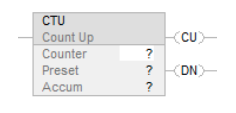
\includegraphics[width=3in]{CTU}}
\caption{Count up instruction}
\label{fig:CTU}
\end{figure}

The field beside the word counter is where you are to type the name of the COUNTER type tag you have created. The preset is the value which you would like to count up to. So, in this case you are counting up to the value 7. So, the preset should be 7. You can enter the value 7 directly into the preset field. 

The .DN bit which is part of the COUNTER type tag associated with the CTU instruction will be false until the counter value reaches the preset value. When the count value reaches the preset value, the .DN bit will become true. The .DN bit should be useful in deciding when to turn on \verb|Shift_Goal_Met|.

\aside{If you wanted to programmatically set the the preset value, you can do so by moving a value into the .PRE attribute which is a part of the COUNTER type tag associated with the timer instruction.}

To reset the counter, you will use a reset instruction (RES). This should be controlled by the \verb|Reset_Counter| signal.


\subsection{The Inputs and Outputs}

To access any of the signals listed in \tableautorefname \ref{Table:Lab5_1Attributes}, use the syntax \verb|Lab5_1.| followed by the attribute name. 

\begin{table}[h]
\centering
\caption{Attributes available in Lab5\textunderscore 1}
\label{Table:Lab5_1Attributes}
\begin{tabular}{c c c}
\toprule
Attribute Name & Data Type & Type\\
\midrule
\verb|Start_Transfer| & Bool & Output \\
\verb|Reset_Counter| & Bool & Output \\
\midrule
\verb|Current_Count| & Dint & Input\\
\verb|Shift_Goal_Met| & Bool & Input\\
\bottomrule
\end{tabular}
\end{table}

Write the appropriate logic in the associated rung in the PLC file.

\TASignatureSlot


\section{Challenge - The Maze Runner}

This section corresponds to the \verb|Lab5_2| object in the Lab5 PLC file.
\\ 
\\

This week the challenge activity is going to be a bit \textit{time} consuming (Pun!). This week the contest organizers decided that each contest will have to write a ladder logic program to guide a ball through a maze... automatically! The maze and the ball will appear on the HMI and you have to make the ball successfully navigate the maze!

\subsection{How should the logic work?}

The logic might seem tough at first glance but it's nothing you can't handle. The way to solve this problem is by writing a bit latch sequence. Each step in the sequence will control a timer and should turn on the appropriate direction control from \tableautorefname \ref{Table:Lab5_2Attributes}. You stay on that step until the timer completes. Then you move on to the next step. 
Hint: You will need one step for each change in direction that that the gold ball must make. ie. if there were 3 turns, then you would need a sequence with 3 steps. 

Hint: The length of time that each step should be on will be a bit of a guessing game. You'll have to figure out how long it takes for the ball to travel from where it starts to where you want it to be.

As a further requirement, when the \verb|Reset| becomes true you must unlatch all the steps in your sequence. When \verb|Go| becomes true the sequence should start and continue until the \verb|Reset| becomes true. Follow the approach to bit latch sequencing that has been discussed in lecture.

Hint: You will need to use timers to accomplish this task, obviously. You can complete it with either the TON timer or the RTO timer. 

\subsection{The Inputs and Outputs}

To access any of the signals listed in \tableautorefname \ref{Table:Lab5_2Attributes}, use the syntax \verb|Lab5_2.| followed by the attribute name. 

\begin{table}[h]
\centering
\caption{Attributes available in Lab5\textunderscore 2}
\label{Table:Lab5_2Attributes}
\begin{tabular}{c c c}
\toprule
Attribute Name & Data Type & Type\\
\midrule
\verb|Go| & Bool & Output \\
\verb|Reset| & Bool & Output \\
\midrule
\verb|Go_Up| & Dint & Input\\
\verb|Go_Down| & Bool & Input\\
\verb|Go_Left| & Bool & Input\\
\verb|Go_Right| & Bool & Input\\
\bottomrule
\end{tabular}
\end{table}

Write the appropriate logic in the associated rung in the PLC file.

\TASignatureSlot



\section{Double Challenge - Simple Waveform}

This week we have a rare double challenge. For the second challenge you are to use timers to make the waveform shown in \figureautorefname \ref{fig:SquareWave} appear in the axes on the HMI. However, the period of the square wave should be editable from the HMI. 

\begin{figure}
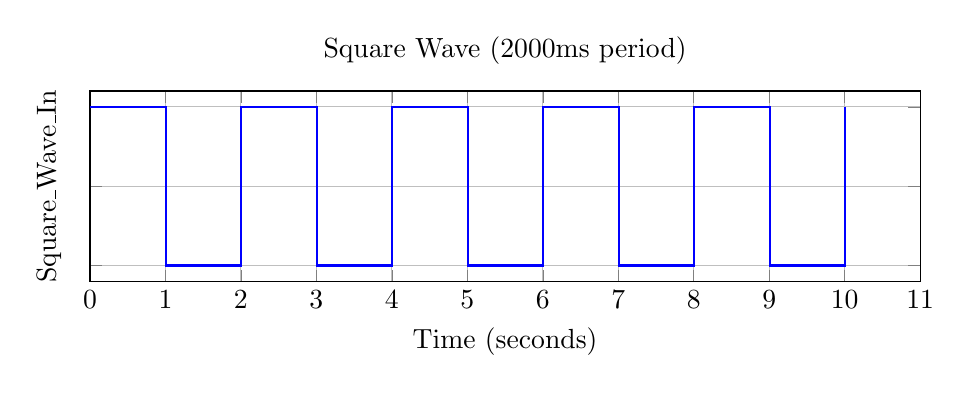
\begin{tikzpicture}
\begin{axis}[grid=both,xmin=0,width=\columnwidth,height=4cm,
title={Square Wave (2000ms period)},xlabel={Time (seconds)},ylabel=Square\_Wave\_In,
yticklabels={,,}]
\addplot+[thick,const plot, no marks,samples at={0,.01,...,10}] {(mod(x,2)>(2*0.5)?0:1)};
\end{axis}
\end{tikzpicture}
\caption{Square Waveform with a 2 second (2000 ms) period}
\label{fig:SquareWave}
\end{figure}

\subsection{How should the logic work?}

The axes shown on the HMI are continuously plotting the state of the \verb|Lab5_3| attribute called \verb|Square_Wave_In|. So, to make a squarewave appear on the axes, you must set \verb|Square_Wave_In| to true for an amount of time equal to one half of the period and then set the tag false for the same amount of time.

There is a field on the HMI that allows the user to edit the value stored in the \verb|Lab5_3| attribute called \verb|Period|. The value stored in this tag should be used as the period for your square wave.

\subsection{The Inputs and Outputs}

To access any of the signals listed in \tableautorefname \ref{Table:Lab5_3Attributes}, use the syntax \verb|Lab5_3.| followed by the attribute name. 

\begin{table}[h]
\centering
\caption{Attributes available in Lab5\textunderscore 3}
\label{Table:Lab5_3Attributes}
\begin{tabular}{c c c}
\toprule
Attribute Name & Data Type & Type\\
\midrule
\verb|Period| & Real & Output \\
\midrule
\verb|Square_Wave_In| & Bool & Input\\
\bottomrule
\end{tabular}
\end{table}

\TASignatureSlot


\begin{samepage}
\begin{figure}[h]
\centering
\textbf{Open Parameters and Local Tags}\par \medskip
\frame{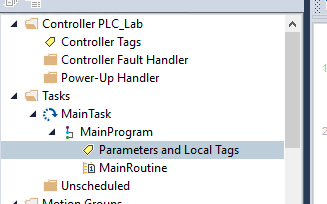
\includegraphics[width=3.2in]{BooleanTagCreation1}}
\caption{First step to creating a new boolean tag}
\label{fig:BooleanTagCreation1_l45}
\end{figure}



\begin{figure}[h]
\centering
\textbf{Create new Boolean Tag}\par \medskip
\frame{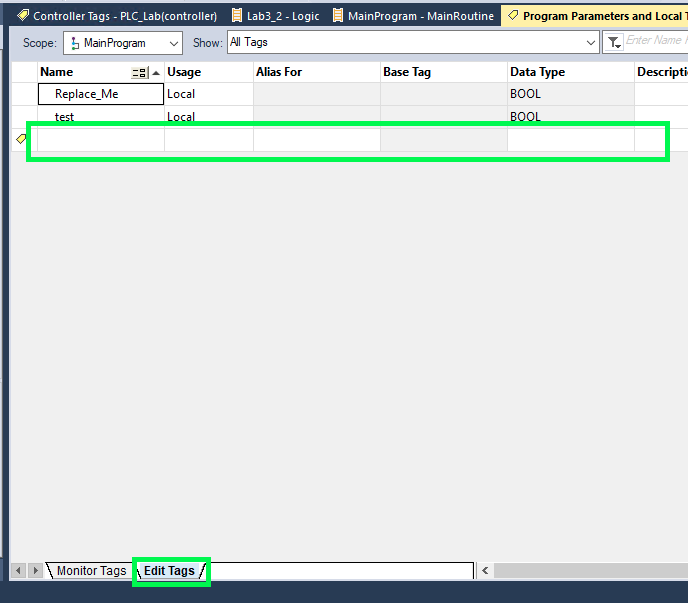
\includegraphics[width=3in]{EditTags}}
\caption{Second and Third step to creating a new boolean tag}
\label{fig:EditTags_l45}
\end{figure}

\section{How to create a boolean tag}
\label{Section:BooleanTag_l45}


To create another boolean tag to store the result of a boolean operation. Go to the left hand controller organizer menu. Under Main Program, double the item named Parameters and Local Tags. Refer to \figureautorefname \ref{fig:BooleanTagCreation1_l45}.



Next, in the window that appears insure that you are on the edit tab of the parameters and tags window. In \figureautorefname \ref{fig:EditTags_l45} you can see that the edit tab is in a green box for visibility at the bottom left. 

Finally, in the bottom entry in the list of tags enter the details for the tag that you are creating. The only two items that you should enter are the name and the datatype. The name must be a name that is not already taken and the datatype must be BOOL.
\end{samepage}
